\documentclass[]{article}

% \usepackage{lmodern}
% \usepackage{amssymb,amsmath}
% \usepackage[T1]{fontenc}
\usepackage[utf8]{inputenc}
\usepackage{microtype}
\usepackage{longtable,booktabs}
\usepackage[unicode=true]{hyperref}
\usepackage{graphicx}
\usepackage{lscape}
\usepackage{titlepage}
\usepackage{listings}
\usepackage{tabularx}




\begin{document}
\maketitlepage
%\section{Ontology}

\abstract{
\noindent
We are building an application which allows the user to keep track of the amount of calories that he/she eats a day.  The application provides a way to track the desired amount of food the user should eat in order to stay on the same weight. Based on the amount of calories the user needs, some recipes are proposed. The user could provide a desired weight, which will lead to an adaptation of the needed calories intake.}

\section{Introduction}
In this report, we look back at the previous assignments and criticise our work. We look back at our database, the ontology made with the entire group and how we map the ontology to our database. We also made a non-trivial demonstrator. 

\newpage

\section{Conceptual schema}
  \begin{figure} [h!]
     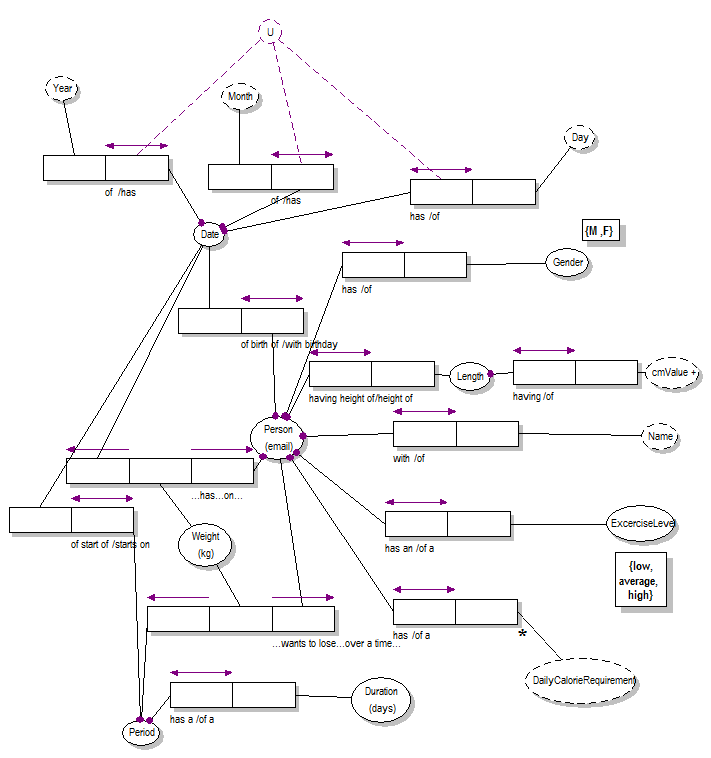
\includegraphics[width = 1.3\textwidth]{image/Person} 
     \caption{ORM of a person}
     \label{fig:twotier}
  \end{figure}
  \begin{figure} [h!]
     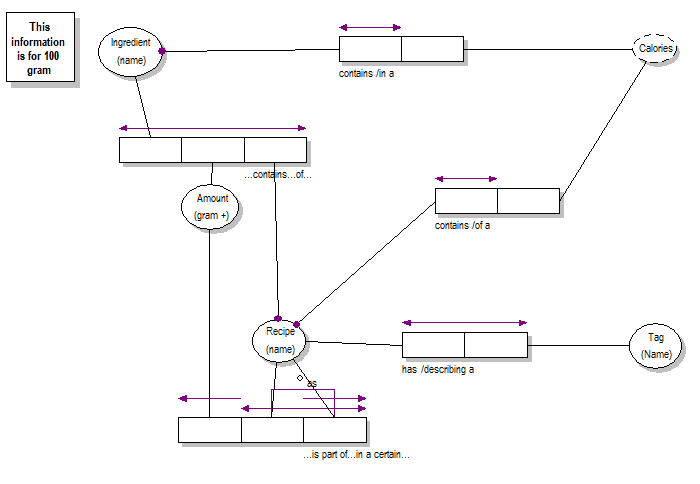
\includegraphics[width = 1.3\textwidth]{image/Recipe} 
     \caption{ORM of a Recipe}
     \label{fig:twotier}
  \end{figure}
\newpage

\subsection{Person} 

We base our application on a person which has as unique identifier an e-mail address. We provide basic information about the user like its  name, height in centimeters, gender, birth date. The gender of a user can be either female or male. A user has an exercise level, this can be high, low or average. This exercise level is important since the amount of calories a user needs in a day is dependent on the amount of exercise the person does. An active person will need a higher amount of calories in a day. Since the application needs to be able to show the fluctuation of the weight of a person, we keep track of how much a person weighs on a specific date. In order to calculate the daily amount of calories the user needs in order to stay on the same weight, we use the following formula: \newline
Basal Metabolic Rate (BMR) of a man= 10 * weight(kg) + 6.25 * height(cm) - 5 * age(y) + 5 \newline
Basal Metabolic Rate of a  woman = 10 * weight(kg) + 6.25 * height(cm) - 5 * age(y) - 161 \newline
In order to calculate the amount of calories a person needs we need to multiply this BMR with 1.3 if the exercise level of the person is light, multiply it with 1.6 if the exercise level is average and multiply it with 2.1 if the exercise level is high. The user's latest weight is used as the weight. This daily calorie amount is derived and not stored. A user also has the possibility to give a weight loss/gain amount, starting at a specific date for a period of days. Then the weight in the formula to calculate the needed calorie amount is adapted on the desired weight. 

\subsection{Ingredient}
The application has a list of ingredients, identified by their name. It also keep track of the amount of calories for 100 gram of the ingredient. An ingredient can be part of a recipe. In that case we also keep track of how much of the ingredient is needed.

\subsection{Recipe}
 A recipe has an amount of calories, which is the sum of all ingredients with their calories. Recipes can be easily found with a tag. This tag can be general and includes for instance breakfast but also more specific, for example; Chinese or Italian. A recipe can be part of another recipe for example the recipe for spaghetti sauce is part of the recipe for lasagna. In that case we also keep track of the amount of the recipe that is needed.   


\section{Database}
Based on this conceptual schema, a relational database schema was created. For this we used a MySQL relational database.As seen in the SQL statement, we used id's to create primary keys for the different concepts (person, recipe, ingredient and tag). This because it is more efficient and clearer to reference different concepts in the relation tables. These are then used as primary keys within the different relations among the concepts. In the persons table a few encodings are used. For one gender is marked by a single character m or f for either male or female. The level of exercise is encoded as an integer from low to high between 1 and 3.\\
\textbf{A dump with test data is also included in the deliverables. MOET DIT ER NOGMAALS STAAN??}

\section{Ontology}

\subsection{Organization}

In order to be able to communicate easily between the different groups we decided, after some initial contact on Facebook, to create a slack channel. This channel was created by Sander Lenearts and at least one person from each group was contacted so all the groups and all their members could join. This slack channel has as an advantage that it was possible to start an initial discussion during the vacation period without having to have everybody physically present at the same place. It was also possible to discus between the food and exercise groups, while providing the option to pin certain decisions and files.\\ \\
We also used Google Doc files that allows for collaboration on a single document. This was used to type out the glossaries, definitions and conceptual schema's.

\subsection{Meetings}

In the first meeting that took place on slack. We wanted to create a global ontology. The only thing that both the food groups and the exercises groups had in common was energy. We decided on a definition that both had a relationship to food and to exercises without getting too technical. Another point of discussion was the unit. Some people wanted to have the SI unit (Joule) but since the unit calories is more widely used, it was decided to use calories as unit. Since there \textbf{where} no more commonalities, we decided to work with the food group separately. This was done in a different slack channel \textbf{where} each group was identified using a separate avatar. 
\newline
\newline
\noindent
The second slack meeting, for the food team, there was at least one member of every group besides group 8. We started with a definition for an Ingredient. A huge point of discussion was whether an ingredient had a brand. Group 5 really wanted this incorporated while this was the only group that needed this aspect. It was proposed that the brand could be part of a more specialised ontology but group 5 didn't agree with this so it was decided that brands would be part of it but, clearly stating that they \textbf{where} an optional property. Since slack has as drawback that it doesn't keep the complete channel history (in the free version) and since discussions on slack can be rather uncoordinated we decided to have the next meeting face to face. 
\newline
\newline
\noindent
Every group had to prepare a glossary and search for entities in their database. During this meeting, that took place Monday 11 April in the morning, all groups but one, group 8, \textbf{where} represented by at least one member. Group 8 did not reply in the slack-channel, the Facebook chat or on the forum on PointCarr\'e. We discussed other ways of contacting them, and decided we would personally contact them during another class. During this meeting we discussed the first food ontology. There was a discussion about whether only to incorporate calories or if other nutritious values \textbf{where} necessary as well. In the end we decided to go with the definition that group 7 proposed since every group was able to map on this definition and since this was the design that was general enough so that the ontology could be easier to reuse. The incorporation of recipe, food and ingredient, and their relation was one of the easiest to decide on. Furthermore we discussed that everybody had some kind of concept to describe either ingredients or recipes, tags in our case. But since the definition of this was so different for each group we settled on not including them at this point in our ontology and we noted that we can always come back to it. During this meeting the focus however did seem to be a lot on how our databases \textbf{where} designed and sometimes group 5 did seem to focus too much on their specific implementation. After agreeing on most definitions and almost finishing the basic ontology, someone noticed that calories is not a nutritional value. We had a discussion whether we should change it and put calorie in the ingredient entity or leave it that way. Where group 5 proposed to put calories in ingredients and have an extra data property that would enable us to use the energetic value of an ingredient in joule or in kCal. Because calories did fit our personal definition of nutritional values, we left it the way we first agreed to it because every group could map onto this ontology. The collaboration went good and we had one person typing our glossary in a Google doc while somebody else drew the different entities on the blackboard. 
\newline
\newline
\noindent
During the evening meeting of Monday 11 April, every group was present but group 8. During this meeting we had the intend to put the ontology in  WebProtégé. We encountered some difficulties with the platform and decided to ask for more information and get together another day. 
\newline
\newline
\noindent
We tried having another meeting on Wednesday 13 April where group 2 and group 1 tried putting the ontology in WebProtégé. Since we still encountered problems we decided to send another mail for more information and ask extra information during the next class of Open Information Systems. 
\newline
\newline
\noindent
During the meeting of Monday 18 April, after having asked questions during the classes that day, all groups \textbf{where} present. We put the ontology in the local version of Protégé. Furthermore we had an extra discussion since we didn't want to have calories in the nutritional value since we didn't like the fact that calories \textbf{wheren}'t in fact nutritional values. Group 5 also brought up that they didn't like the relationship with amount/nutritional value since it was too complex. They proposed (again) to have an extra data property \emph{energy} on the ingredient class. After hearing the arguments it was decided to change the name, since calories aren't nutrients. But to keep the relationship with amount(changed name to quantity since this is more informative)/nutritional value since this one is more general. We like to note that while groups 8 and 4 where present they didn't have any input.\\ \\
We also faced the issue of adding an extra class between ingredient and nutritional value. This is not strictly necessary but because we also had a \emph{linking} class between recipe and ingredient we decided to add this as well. This because otherwise ingredient class would have a data property amount, which is not very generic as other applications might be interested in only the ingredient class. During this meeting some name changes where made because they where clearer.

\subsection{Team Organization}

Since Arno De Witte was on vacation during spring break, both Jolien Declerck and Silke Verhaeghe attended the first two slack meetings and the first real life meeting. In case we \textbf{wheren}'t sure of certain aspects we could always reach Arno and a global overview of the decisions was given after each meeting. For the rest of the meetings everyone of our group was present. Arno was the one to apply the remarks of the teacher to our current database/Conceptual schema. Writing the report was a group effort. \todo{Uitbreiden met wat er laatste stretch nog gedaan is}

\subsection{Other discussions}
We discussed what other groups had in common with our proposal. Because there where no things that where worthwhile exchanging we did not add an extra ontology.
\newline
\newline
\noindent
We had the discussion with all of the groups whether or not we should exchange information about our users or the accounts. We did not see any benefits and for privacy reasons for the user we decided not to exchange user information and therefore not include this in the ontology. \todo{aanpassen ontology, namespaces}

\subsection{Ontology explained}
The ontology is centred around the ingredient class. An ingredient was the thing we all had in common to start with. Ingredients have nutritional values like sugar, salt and calories, specified in the list of nutritive values. We have decided to make an extra class nutritive value to specify this. Because we need to be able to have multiple nutritive values for one ingredient, we have added the nutritive value quantity. This was necessary for some of the groups in order to be able to map to the ontology. Here you can specify the quantity specified for a nutritive value for 100 gram.
\\ \\
Ingredients can also be combined into a recipe. We have also added an ingredient quantity class for the same reason we added the nutritive value quantity. A recipe can have multiple ingredients combined. The ingredient quantity class specifies the quantity needed for the ingredient in a specific recipe. We have also provided the unit of quantity. Combining some ingredients result into a recipe. The result of a recipe is something that we can eat so we have classified this as food. There is also a possibility to provide steps in order to complete a recipe. Steps consists of an ordering number and the description of the step. 
\\ \\
Because we have made this decision, all groups can map onto it. In our case, not every ingredient is combined into a recipe but it is still food. Therefore we can say for example, one apple is the ingredient for eating an apple, it does not specify any steps. Via this way we can say that an apple is a food.
\\ \\
We did not add a link between food and ingredient. This is because in the Open World Assumption a food can also be an ingredient. Initially it was provided to add a link but some groups protested because they did not see the benefit of it so we left it out. 

\section{Glossary}
\textit{Recipe} \\
A collection of ingredients and/or the steps necessary to combine the ingredients into some food. It contains a list of ingredients with their quantity, a list of steps to complete the recipe and a link to food. \\ \\
\textit{Food} \\
Any substance that can be eaten or drunk. When consumed, it provides a nutrition. Food can be an ingredient or the result of a recipe. It only has a name. \\ \\
\textit{Ingredient} \\
An ingredient is a substance containing nutrients; an ingredient can be a food. It contains an optional brand, a name and a list of nutritive values with their quantity. \\ \\
\textit{Ingredient Quantity} \\
The link between a recipe and an ingredient. 
It depicts the amount of some ingredient necessary to complete a recipe.
It contains a reference to the ingredient, a quantity and the unit for which the quantity is specified. This can be liter, a table spoon or something similar.
\\ \\
\textit{Nutritive value} \\
A substance that provides nourishment essential for the maintenance of life and for growth. For example fat, sugar, carbohydrate, protein, sodium. This contains only a name. \\ \\
\textit{Nutritive Value Quantity} \\
The link between a nutrition and an ingredient. 
It depicts the amount of some nutrient per 100 gram of some ingredient. This contains an ID of nutritive value, a quantity and the unit for which the quantity is specified.\\ \\
\textit{Recipe Step} \\
A step in the preparation process of a recipe. A step has a ordering number starting from 1. A step has a number for ordering and a string as a human readable description. This contains an order number which specifies the order of the steps and a description.

\section{Mapping database to ontology}
Because we want a lot of data where we can query on, we asked the other food-groups to exchange their triples. Some exercise groups also wanted to use the triples of the food groups. Therefore, our group put messages on the slack channel, on the Facebook group and on the pointcarré-forum of the course. Although we thought that it could benefit other groups to, to exchange the information, we did not get the response we've expected. This could be because some groups did not had their triples ready or they did not saw the message although we put it on three different media.\todo{nog iets over hoe we dat zelf gedaan hebben, recipe name en geen steps enzo?}

Only group 1 and group 5 asked to use our triples for the food-groups and one exercise group wanted to use our triples to. We have send them our ttl-file. 
\section{Non-trivial demonstrator}
Our demonstration allows to formulate a number of health and dieting constraints (has to consume a number of calories, cant eat too much salt, is allergic to nuts, ...) and search for fitting recipes. Our demonstration allows to easily fill in these constraints and suggests a number of recipes that fit these needs. Users can combine constraints in a "and-or-not" kind of fashion. For example a user cannot eat too much fat combined with too much sugar, he is also allergic to bananas. This would result in a rule; fat lower than 30g or sugar lower than 20g and no bananas. Additional to this user can express preferences, for example a user dislikes broccoli but likes fries. Recipes with broccoli will be ranked lower than recipes with fries.

This demonstration uses the developed ontology and thus also databases of other teams. This because the ontology provides the ingredients for each recipe as well as their nutritive values. In our original application (and database) we don't provide nutritive values other than calories. Therefore we will need to query other projects SPARQL endpoints, which will hopefully provide these values. We plan to use a rule system to indicate whether a recipe is favourable, unfavourable or neutral for a certain set of preferences.
\subsection{Rule based languages}
We have looked at two different rule based languages, SPIN and SWRL. Vergeet niet te zeggen da je constraints kan definiëren adhv een sparql CONSTRUCT query!!

\todo{hier komt de vergelijking}
\subsection{Non-trivial demonstrator}
Our demonstrator is implemented as a java application which can be used as a commandline tool. It has dependencies on the jena API\footnote{\url{https://jena.apache.org/}}, SPIN open source API\footnote{\url{http://topbraid.org/spin/api/}} and the Antlr parser library\footnote{\url{http://www.antlr.org/}}. As said in the previous section we used SPIN to implement our demonstrator. For our demonstrator we implemented two SPIN constraints, one to filter recipes that contain a certain ingredient and one to filter recipes that contain too much of a certain nutritive value. These constraint were abstracted using SPIN templates. This allows to use parameters such as the nutrient name or the nutrient value. We also added a parameter to indicate a certain violation level\footnote{\url{http://spinrdf.org/spin.html\#spin-constraint-construct}}. This parameter was used to differentiate between hard and soft constraints. To apply these SPIN constraints, a constraint had to be added to the Recipe class defined in the ontology as shown below:
\begin{lstlisting}[caption=Example of applying constraints in turtle]
ont:Recipe  
  spin:constraint  [ a ont:templateIngre ;
                     ont:parIngredient  "Tomato" ;
                     ont:parWarn        spin:Warning
                   ] ;
  spin:constraint  [ a ont:templateNut ;
                     ont:parNutrient  "Cholesterol" ;
                     ont:parValue     "4"^^xsd:int ;
                     ont:parWarn      spin:Error
                   ] .
\end{lstlisting} 
These applications are added to the model at runtime by the java code. Thereafter all the models containing triples are united and the SPIN constraint check method will produce a list of constraint violations. These are then looped over and divided in hard and soft constraint violations. Then all recipes (except the ones that violate a hard constraint) are queried and displayed to the user.\\
The constraints can be expressed using a simple language which is defined as seen below. With the Antlr library a walker can be generated. In this walker at the end of each constraint, a method is called which adds this constraint to the model. 
\begin{lstlisting}[caption=Example of the constraints file]{Name}
HARD "Cholesterol" < 4 AND
SOFT not "Tomato" 
\end{lstlisting}
There were some issues that occurred during the implementation of the demonstrator. We wanted to allow for a and-or type of chaining of constraints. This was however difficult as the SPIN constraints don't allow for this kind of functionality. A solution would be to define ID's to each constraint and then check within the java code. But the SPIN open source API (which is not documented) does not allow to retrieve additional properties given to a constraint.\\
We also tried to implement different kind of operators for the nutrient constraint (e.g. smaller than, equals). But because the constraints are implemented in SPARQL and it is not possible to use a variables as operator, this was not possible. We tried to use the SPIN SPARQL syntax but the syntax for operators is undocumented (however some operators are shown in the examples) and support for it in the open source API is lacking at this time.\\
For future work this demonstrator could be expanded by adding more constraints (e.g. limiting the amount of steps in a recipe). A larger amount of constraints would indicate that more abstract templates can be defined (now only two separate templates exist). Further more the rule system in SPIN could be used to infer properties (e.g. recipe length).

\section{Reflection}
\todo{DATABASE}

ONTOLOGY
Although every group participated and checked the ontology, we missed something. We forgot to gave a recipe a name. For our group, this was not a problem, because we mapped every recipe as food as well and food contains a name. Some other groups also complained again about the nutritional values and the quantity of them. Because this is not something we have, this was not a problem for our group. 

MAPPING

\subsection{Non-trivial demonstrator}
When looking into SPIN it seemed a perfect fit for the demonstrator we wanted to implement. However the lack of documentation of the open source API and the lack of documentation surrounding the operators made implementing all of our goals impossible. SPIN is a good fit for these kind of projects because of its relation with SPARQL, but the implementation and documentation of the API could be a lot better at this point in time.

\section*{References}
http://www.bbc.co.uk/ontologies/fo\newline
http://data.lirmm.fr/ontologies/food\#Food\newline
http://dbpedia.org/ontology/Food \newline
http://dbpedia.org/ontology/ingredient\newline
http://semanticdiet.com/ontology.event \newline
http://dbpedia.org/ontology/Person \newline


http://starpc14.vub.ac.be:8080/webprotege
\end{document}
